%Paper template for the MEC-E2010 Computational Fluid Modelling
%course. Authored by Theo Eklund.
%In case of any problems, contact the teacher in charge
%Tommi Mikkola (tommi.mikkola@aalto.fi)
\documentclass{cfm_paper} %extarticle class needed to use 9pt font size
\addbibresource{references.bib} %This should be your bib file

\graphicspath{{fig/}}

\begin{document} %Change these according to your background etc.

\title{Title of your paper}
\author{Firstname Lastname}
\university{Aalto University}
\school{School of xxx}
\programme{Master's/Doctoral programme on yyy}

\maketitle

\begin{abstract}
This is the abstract of the paper explaining briefly the topic and motivation of the work, the modelling approach, main results and conclusions.
\end{abstract}


% \begin{strip}
% \begin{center}
%     {\huge 
%     Title of your paper
%     } \vspace{0.4cm} \\
%     Firstname Lastname \\
%    Aalto University  \\
%     School of xxx \\
%     Master's/Doctoral programme on yyy
%     \vspace{0.4cm}
% \end{center}
% \end{strip}

% \textbf{Abstract:
% This is the abstract of the paper explaining briefly the topic and motivation of the work, the modelling approach, main results and conclusions.
% } %Abstract in bold, therefore the \textbf code

\section*{INTRODUCTION} %The * implies that there should be no numbering
This is template for the final paper on the MEC-E2010 Computational Fluid dynamics course. The different elements for the layout of the paper are provided in the following. The paper should have sections on introduction, modelling approach, case setup, results and discussion and conclusion.

\section*{MARGINS AND PAPER LAYOUT}
The paper size is A4 with 2cm margins on all sides (top, bottom, left, right). The layout is two column layout with 1cm separation between the columns. 

\section*{FONTS}
The font for all elements of the text is Times New Roman. The font size for the main body of text is 9pt (the Normal style in the template). The font size for the main headings is 9pt and these are type set in all caps (the Heading 1 style in the template)

\subsection*{Subheadings}
The font for the subheadings is bold font in 9pt size (the Head-ing 2 style in the template). You should not use more than two levels of headings in your paper.

\section*{EQUATIONS}
Equations should be type set centered and numbered consecutively.
\begin{equation} %This command will automatically put the number in parentheses at the end of the row
    A = \pi r^2
\end{equation}
The numbering should be flush to the right edge of the column. You can get this with the equations style, which has a centered and right justified tab stops for the equation and the equation number respectively.
\begin{equation}
    (1+x)^n = 1 + \frac{nx}{1!}+\frac{n(n-1)x^2}{2!}+...
\end{equation}

\section*{TABLES}
Tables can be included as either one column or two column tables. Two column tables should be placed either at the top or bottom of the page, centered, typeset in the same font as the main text and numbered consecutively. The table should not have any borders, but there should be a horizontal line separating the column headings.


%Multicols does not support float objects. Therefore, one workaround is to use \begin{center}, which centers everything and then you can use the \captionof command to add the proper caption. 
    \begin{table}[h]
\caption{Example of a table and table caption.} %This creates a caption for a table
\label{tab:ExampleTable}
\begin{tabularx}{\columnwidth}{XXX} %This command ensures that the table is always as wide as the column allows it to be. ONLY WORKS WITH "X", no other letter macros.
\toprule
Column 1 & Column 2 & Column 3 \\
\midrule %This is the horizontal line after the table headers.
Item 1   & Item 2   & Item 3   \\
Item a   & Item b   & Item c   \\
\bottomrule
\end{tabularx}
\end{table}

There should be one empty line after the table to separate it from the rest of the text.
% \columnbreak %This ensure that the text after this will flow into the next column. Use this to tidy up columns and overall layout when finishing the report.
\section*{FIGURES}
Figures can be included as either one column or two column figures. Two column figures should be placed either at the top or bottom of the page, centered, typeset in the same font as the main text and numbered consecutively.

%Use a \begin{figure} with an \includegraphics[width=\columnwidth] to insert an image with the exact width of the column
\begin{figure}
    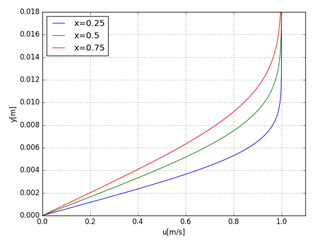
\includegraphics[width = \columnwidth]{cfm_test.png}
    \caption{Example of a figure and a figure caption} %Creates a figure caption.
    \label{fig:ExampleFigure}
\end{figure}

Pay attention to the size of the text in the figures. The text size should be such that it is easily legible. Avoid excessive margins around the figure and crop the figure accordingly if necessary.

\section*{REFERENCES}
The list of references is placed at the end of the paper with a main heading REFERENCES. The list should be organized in alphabetical order based on the name of the first author and items should be numbered consecutively. In the text you should cite the number in square brackets e.g. \cite{Hanninen2016, Tu2012}. %Cite is used to cite the sources which are located in the references.bib file.
Examples of references are shown in the following.

\printbibliography[title={REFERENCES}] %This prints the bibliography with the title "REFERENCES".

\end{document}
